% Title
\title{DVA227 Grupp 4 - Rapport}

% Document type
\documentclass[11pt, titlepage, a4paper]{article}

% Preamble
% ==================== Packages ====================
% Character Encoding
\usepackage[T1]{fontenc}
\usepackage[utf8]{inputenc}
\usepackage{lmodern}
\usepackage[swedish]{babel} % <-- Change language used here. Rememeber to clean all the aux files before building document.
\usepackage{csquotes}
\usepackage{microtype}

% Bibliography & References Formatting
\usepackage[style=ieee,backend=biber,dateabbrev=false]{biblatex}

% Appendices Formatting
\usepackage[titletoc,title]{appendix}
%\renewcommand\appendixtocname{Bilagor}     % <-- If needed to manually change appendice names
%\renewcommand\appendixpagename{Bilagor}    % <-- If needed to manually change appendice names

% Text Formatting
\usepackage{marginnote}
\usepackage[absolute]{textpos}
\sloppy

% Document Formatting
\usepackage{fancyhdr}
\usepackage{enumerate}
\usepackage{enumitem}
\usepackage{listings}
\renewcommand{\lstlistlistingname}{Listor}   % If needed to manually change list of lists's name in ToC.
\renewcommand{\lstlistingname}{Lista}        % If needed to manually change list's name in document.
\usepackage[margin=3cm]{geometry}
\usepackage[section]{placeins}

% List code style
\lstset{
    backgroundcolor=\color[rgb]{0.92,0.92,0.92},
    basicstyle=\ttfamily,
    columns=fullflexible,
    keepspaces=true,
    frame=single,
    showspaces=false,
    showstringspaces=false,
    showtabs=false,
    tabsize=2,
    captionpos=b,
    breaklines=false,
    keywordstyle=\color[rgb]{0,0,1},
    commentstyle=\color[rgb]{0.133,0.545,0.133}
}

% Urls & Hyperref
\usepackage{url}
\usepackage[pdfborder={0 0 0}, colorlinks=true, urlcolor=blue, citecolor=red, bookmarks=false]{hyperref}

% Image and Table Formatting
\usepackage{tabularx}
\usepackage{caption}
\usepackage{graphicx}
\usepackage{array}
\usepackage{diagbox}
\usepackage{chngcntr}
\usepackage{multirow}
\usepackage{color, colortbl}

% Tikz
\usepackage{tikz}

% Math
\usepackage{amsmath}
\usepackage{amsfonts}
\usepackage{mathtools}
\usepackage{bm}

% Other
\usepackage{lipsum}
\usepackage{datetime}
\bibliography{static/biblio}

%============================== Custom macros for document

%=============== Front page info
%% Logo info
\def\tLogoLocation{static/MDHlogga.png}
\def\tLogoWidth{15mm}

%% School info
\def\tSchoolName{Mälardalen University}
\def\tAcademyName{School of Innovation, Design and Engineering}     % IDT
\def\tSchoolLocation{Västerås, Sweden}

%% Course info
% Leave the fields for titles, authors and teachers blank if you don't need them.
% e.g. \tTitleThree{}
% They will automatically be hidden on the front page.

\def\tCourseName{DVA227 - Projekt i Nätverksteknik}
\def\tTitleOne{Projekt Bolaget}
\def\tTitleTwo{Projektrapport}     % <-- Set to {} to hide
\def\tTitleThree{Ver 1 Rev 2}   % <-- Set to {} to hide

%% Author info
\def\tAuthorTitle{Grupp 4}     % <-- Set to {} to hide

\def\tAuthorOneName{Mikael Andersson}       % <-- Set to {} to hide
\def\tAuthorOneEmail{man16057@student.mdh.se}
%======
\def\tAuthorTwoName{Vilhelm Beijer}       % <-- Set to {} to hide
\def\tAuthorTwoEmail{vbr16001@student.mdh.se}
%======
\def\tAuthorThreeName{Isak Söderström}      % <-- Set to {} to hide
\def\tAuthorThreeEmail{ism16002@student.mdh.se}
%======
\def\tAuthorFourName{}    % <-- Set to {} to hide
\def\tAuthorFourEmail{}

%% Teacher info
\def\tTeacherOneTitleAndName{Kursansvarig, Lärare \& Examinator: Joakim Rydén}
\def\tTeacherOneEmail{joakim.ryden@mdh.se}
\def\tTeacherOneLocation{\tSchoolName, \tSchoolLocation}
%======
\def\tTeacherTwoTitleAndName{Lärare: Sara Lundahl}  % <-- Set to {} to hide
\def\tTeacherTwoEmail{sara.lundahl@mdh.se}
\def\tTeacherTwoLocation{\tSchoolName, \tSchoolLocation}

%% Misc
\def\tDateDocMade{12 april 2018}     % Use \today or set a date manually

\def\tDates{\begin{tabular}{rl}
        Skapad:     & \tDateDocMade \\
        Uppdaterad: & \today\,\,\currenttime
    \end{tabular}
}

%=============== Document Headers
\def\mLHeader{\tSchoolName}
\def\mRHeader{\tTitleTwo\ - \tTitleThree}
%============================== End of macros

% Page style
\pagestyle{fancy}
\marginparsep = 10pt
\renewcommand*{\marginfont}{\footnotesize}

% Table of Contents
\renewcommand\contentsname{Table of Contents}
\newcommand{\HRule}{\rule{\linewidth}{0.5mm}}
\newcommand{\circR}{\textsuperscript{\textregistered}}

% Document begins
\begin{document}

    % Title
    \hypersetup{pageanchor=false}
    \begin{titlepage}
        \begin{center}
    \begin{figure}[t]
        \includegraphics[width=\tLogoWidth, viewport=0 0 100 100]{\tLogoLocation}
    \end{figure}

    \Large \tSchoolName \\
    \Large \tAcademyName \\
    \Large \tSchoolLocation \\

    \noindent\makebox[\linewidth]{\rule{\textwidth}{0.4pt}} \\ [0.5cm]

    \Large{\tCourseName} \\ [1.0cm]

%============================================================
% Title management

    \Huge \textbf{\underline{\tTitleOne}} \\ [0.5cm]
    \ifx
        \tTitleTwo \empty
            %nothing
        \else
            \huge \textbf{\uppercase{\tTitleTwo}} \\
    \fi
    \ifx
        \tTitleThree \empty
            ~\\ [0.5cm]
        \else
            \huge \textbf{\uppercase{\tTitleThree}} \\ [1cm]
    \fi

%============================================================
% Author management

    \ifx
        \tAuthorTitle \empty
            %nothing
        \else
            \LARGE \textbf{\underline{\smash{\tAuthorTitle}}} \\ [0.2cm]
    \fi
    
    
    \LARGE \tAuthorOneName \\
    \large \href{mailto:\tAuthorOneEmail}{\tAuthorOneEmail} \\
    
    \ifx
        \tAuthorTwoName \empty
            %nothing
        \else
            \LARGE \tAuthorTwoName \\
            \large \href{mailto:\tAuthorTwoEmail}{\tAuthorTwoEmail} \\
    \fi
    \ifx
        \tAuthorThreeName \empty
            %nothing
        \else
            \LARGE \tAuthorThreeName \\
            \large \href{mailto:\tAuthorThreeEmail}{\tAuthorThreeEmail} \\
    \fi
    \ifx
        \tAuthorFourName \empty
            %nothing
        \else
            \LARGE \tAuthorFourName \\
        \large \href{mailto:\tAuthorFourEmail}{\tAuthorFourEmail} \\
    \fi

    \vspace*{\fill}

%============================================================
% Teacher management

    \begin{flushleft}
        \Large \tTeacherOneTitleAndName \\
        \begin{minipage}[t]{0,7\textwidth}
            \large \href{mailto:\tTeacherOneEmail}{\tTeacherOneEmail} \\
            \large \tTeacherOneLocation
        \end{minipage} \\ [0.5cm]

        \ifx
            \tTeacherTwoTitleAndName \empty
                %nothing
            \else
                \Large \tTeacherTwoTitleAndName \\
                \begin{minipage}[t]{0,7\textwidth}
                    \large \href{mailto:\tTeacherTwoEmail}{\tTeacherTwoEmail} \\
                    \large \tTeacherTwoLocation
                \end{minipage} \\ [0.5cm]
        \fi
    \end{flushleft}

%============================================================

    \large \tDate

\end{center}
    \end{titlepage}
    \hypersetup{pageanchor=true}

    % Page style
    \pagestyle{fancy}
    \fancyhead[L]{\mLHeader}
    \fancyhead[R]{\mRHeader}
    \setlength{\headheight}{14pt}
    \fancyfoot[L]{}
    \fancyfoot[R]{}
    \renewcommand{\headrulewidth}{0.4pt}
    \renewcommand{\footrulewidth}{0.4pt}

    % Reset of counters after each section
    \counterwithin{figure}{section}
    \counterwithin{table}{section}
    \counterwithin{lstlisting}{section}

%========================== Table of contents =========================
    \pagenumbering{Roman}
    \hypersetup{linkcolor=black}

    % Table of contents
    \tableofcontents        % <-- Comment out if not needed
    %\newpage

    % List of figures
    \listoffigures          % <-- Comment out if not needed

    % List of tables
    \listoftables           % <-- Comment out if not needed

    % List of lists
    %\lstlistoflistings      % <-- Comment out if not needed

% =========================== Actual Content ==========================
    \newpage
    \pagenumbering{arabic}
% ========== Add your texts here

    \section{Inledning}
I början av februari tilldelades vi ett projekt av Johnny Bergklint på Netsecure. Projektet gick ut på att standardisera nya branch-siter åt ett företag, fortsättningsvis benämnt som \textquotedblleft Bolaget\textquotedblright, som har dessa typer av siter runt om i världen. I denna rapport presenteras resultatet av arbetet kring detta projekt, vilket i stor del går ut på att ta fram designförslag och idéer för att driftsätta nya siter. På grund av sekretessen kring projektägaren kunde inte en fullständigt detaljerad plan levereras, men detta arbetet kan ses som ett embryo till en färdig lösning.

% ##########
\section{Hårdvarulayout}
    Vi har valt att använda produkter från Fortinet då det finns ett partnersamarbete mellan dem och Netsecure. Vad vi kan se är Fortinets utbud väl tillräckligt för den utrustning vi har valt och priset har legat jämnt eller lägre gentemot andra märken för den prestanda som behövts.

\subsection{Minimikrav}
    \begin{itemize}[noitemsep]
        \item Högst 24 personer på varje site.
        \item Högst 6 kontorsenheter t.ex. printers, ip-telefoner.
        \item Högst 2 AP:s på varje site, dessa ska stödja dual-radio (dvs 2.4 Ghz \& 5Ghz)
        \item Varje site har upp till två anslutningar till core siterna.
        \begin{itemize}[noitemsep]
        	\item En krypterad anslutning över internet med hastighet upp till 100 Mbit/s.
            \item En VPN-anslutning över ett privat nätverk som är isolerat från internet med hastighet upp till 50 Mbit/s.
        \end{itemize}
    \end{itemize}
    
    \noindent Efter dessa minimikrav designades följande topologi för siterna, vilket kan ses i Figur \ref{fig:site-topology}:
    \begin{itemize}[noitemsep]
    	\item En FortiGate 60E-PoE router kopplad till ISP och/eller VPN beroende på det lokala förutsättningarna.
        \item En FortiSwitch 124E kopplad till routern för användare.
        \item Två FortiAP 221C access-punkter kopplade direkt till routern med PoE.
    \end{itemize}
    
 	\begin{figure}[htb]
        \centering
        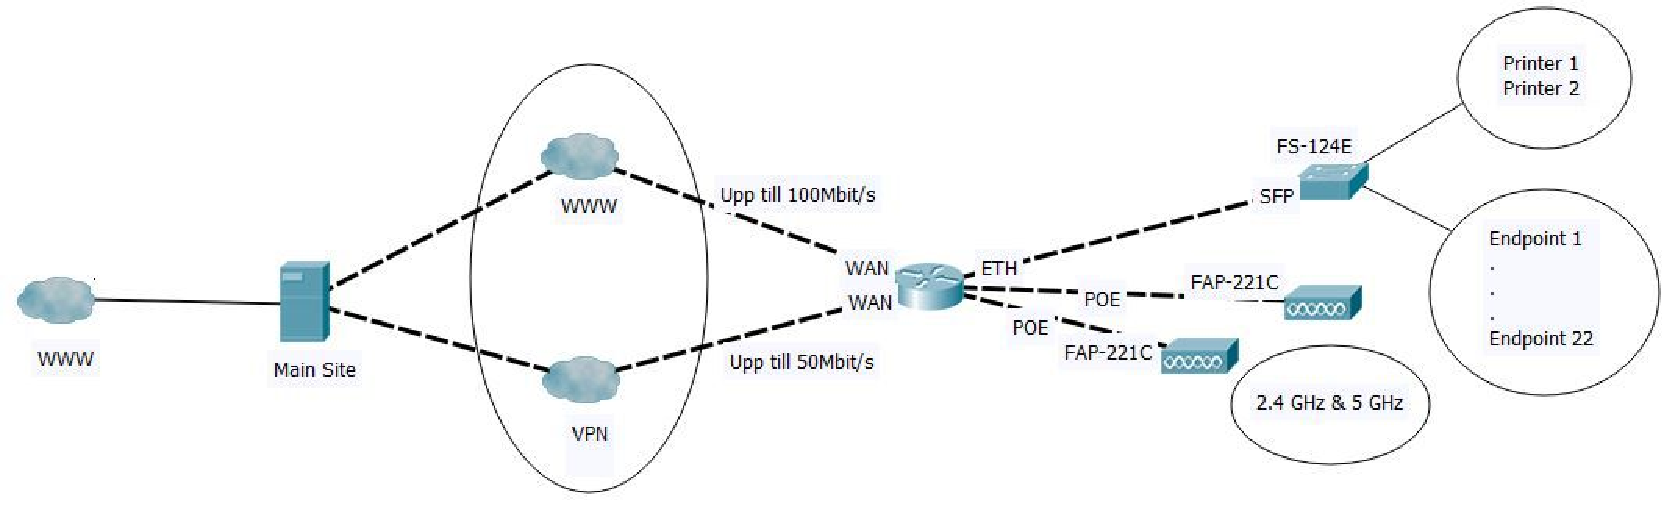
\includegraphics[width=\textwidth]{pics/Topologi_H_rdvara.pdf}
        \caption{Topologi för hårdvarulayout.}
        \label{fig:site-topology}
    \end{figure}

\subsection{Routing \& Brandvägg}
    Routern och brandväggen som valts till projektets lösning är FortiGate 60E-PoE, se Figur \ref{fig:router-60e}. Denna routern valdes för att det är den billigaste router som uppfyller minimikraven på överföringshastigheten även när alla brandväggsfunktioner används. Den har tillräckligt många portar för att täcka de behov som behövs samt PoE som behövs till accesspunkter.
    
    \begin{figure}[htb]
        \centering
        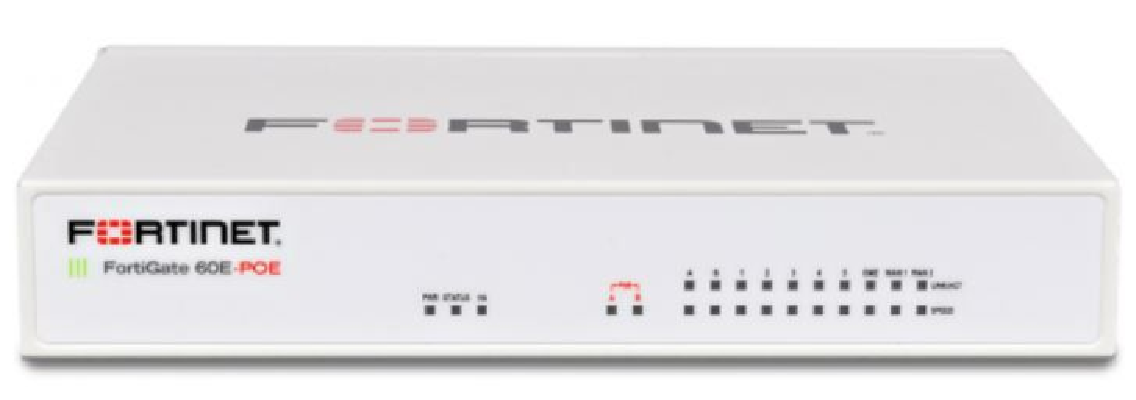
\includegraphics[width=0.95\textwidth, clip, trim={0 0 0 0}]{pics/FortiGate-60E-POE-Frontside.pdf}
        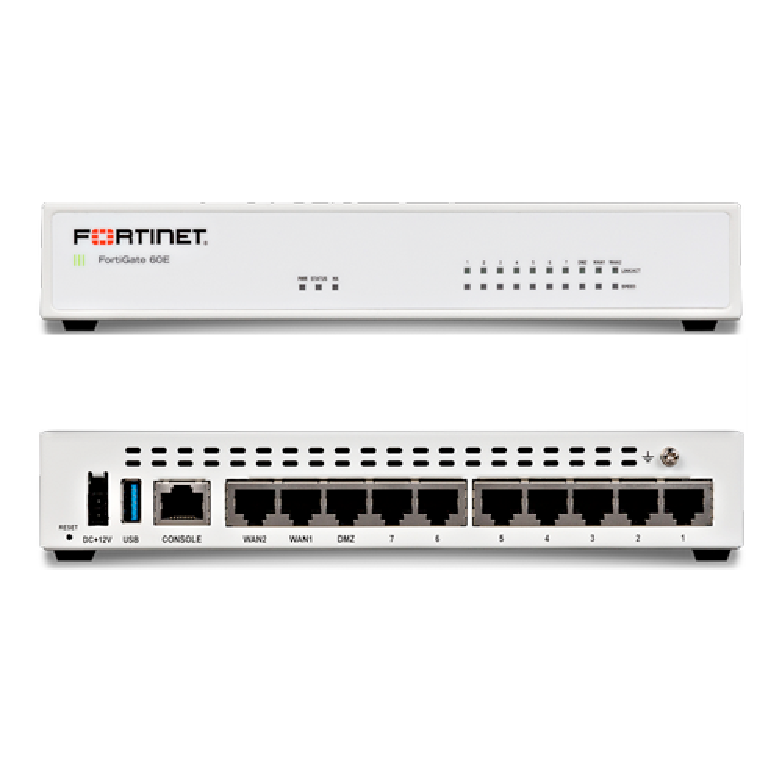
\includegraphics[width=\textwidth, clip, trim={0 3cm 0 6.5cm}]{pics/fortigate-60e-facerear.pdf}
        \caption[FortiGate-60E]{FortiGate 60E-PoE.}
        \label{fig:router-60e}
    \end{figure}

\subsection{Switching}
    FortiSwitch 124E är switchen som valdes och precis som med routern var det priset kontra prestanda som avgjorde valet. FortiSwitch 124E är Fortinets billigaste 24-portars switch och en sådan täcker de maximala antalet användare som kan komma att finnas på vardera site. Switchen kan ses i Figur \ref{fig:switch-124e}.
    
    \begin{figure}[htb]
        \centering
        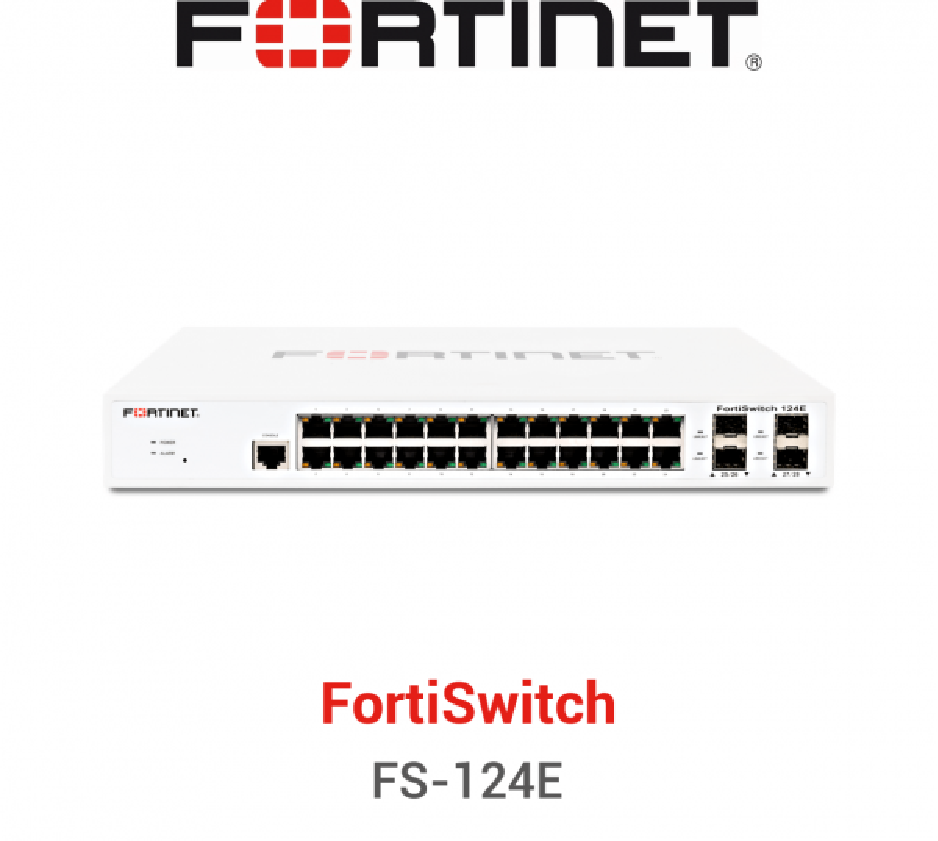
\includegraphics[width=\textwidth,trim={0 5cm 0 5cm}, clip]{pics/FortiSwitch-124E_icon_600x600.pdf}
        \caption{FortiSwitch 124E}
        \label{fig:switch-124e}
    \end{figure}

\newpage
\subsection{Wireless}
    FortiAccessPoint 221C är en av Fortinets enklare trådlösa accesspunkter men innehar tillräckligt med funktionalitet för att täcka de krav som kunden har ställt, exempelvis 2x2 MIMO och dual-radio för att kunna köra både på 2.4Ghz och 5Ghz bandet \cite{FN_FortiAP}. Access-punkten kan ses i Figur \ref{fig:ap-221c}.
    
     \begin{figure}[htb]
        \centering
        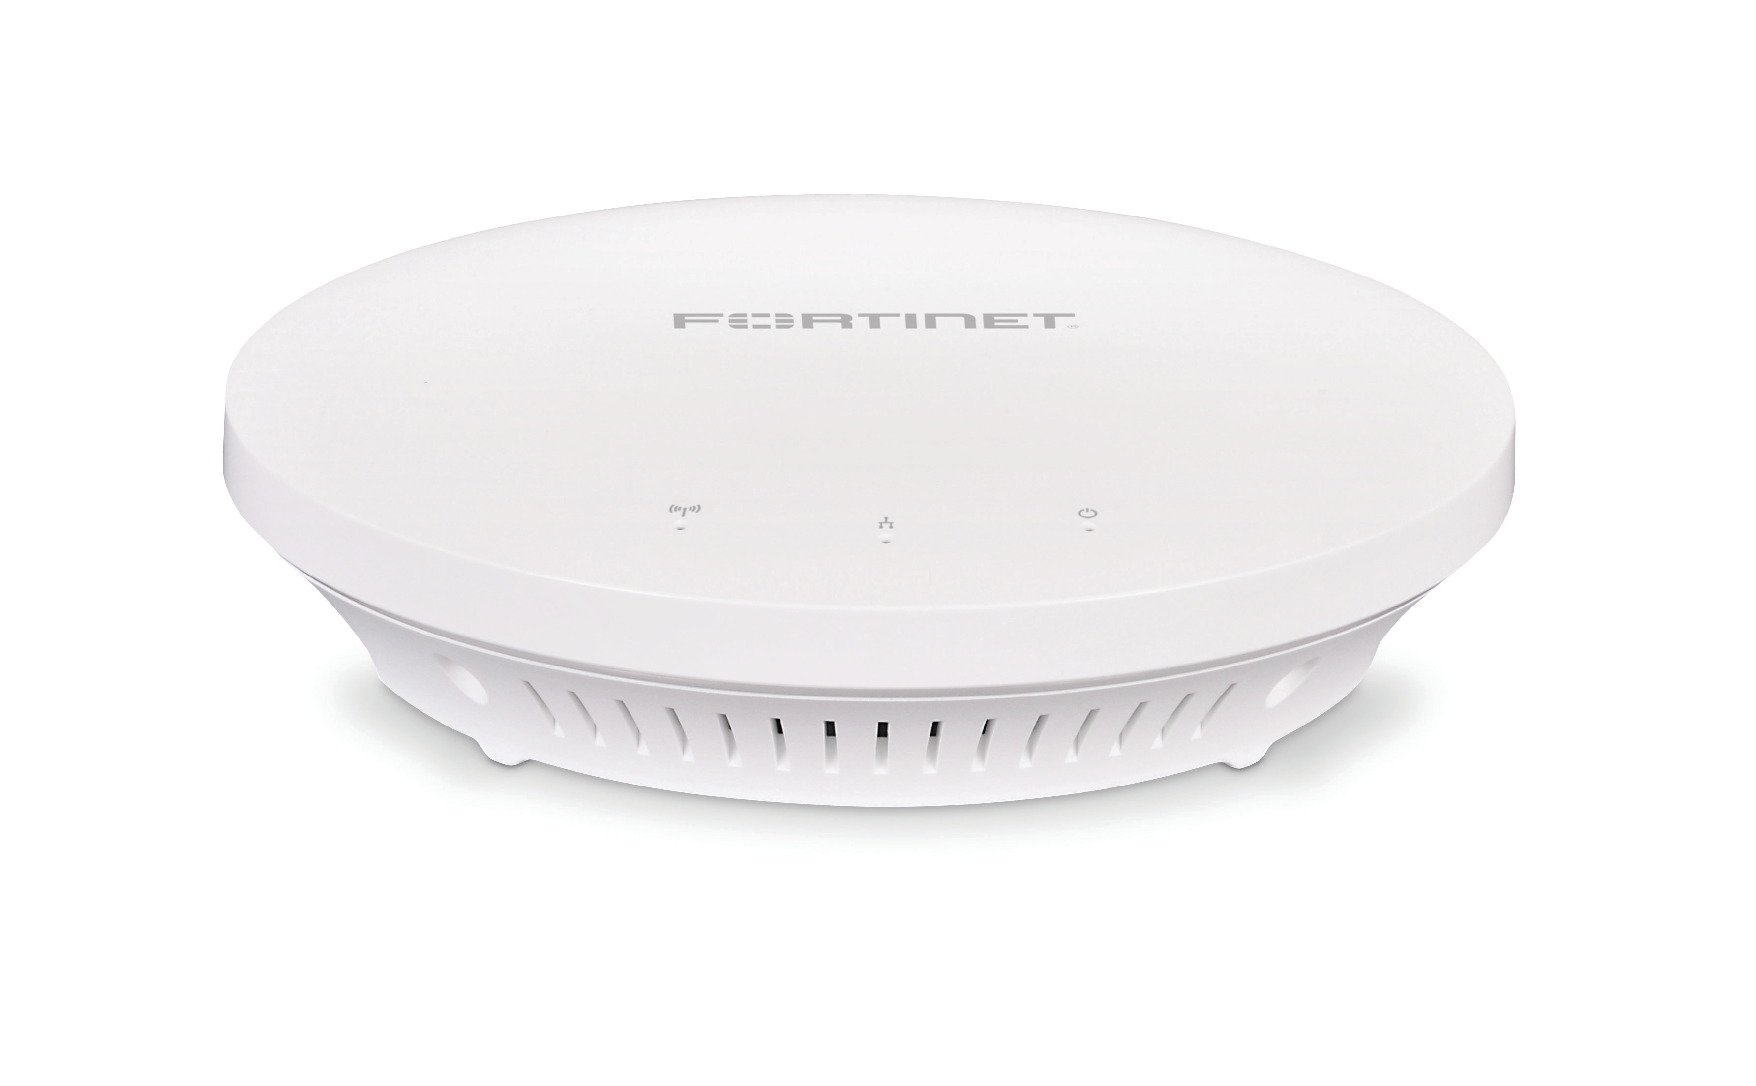
\includegraphics[width=0.8\textwidth,trim={0 3cm 0 1cm}, clip]{pics/FortiAccesspoint-221C.pdf}
        \caption{FortiAccessPoint 221C}
        \label{fig:ap-221c}
    \end{figure}

\subsection{Fysisk Säkerhet}
Vi ger följande rekommendationer för att säkra siternas hårdvara:
    \begin{itemize}[noitemsep]
        \item Låsta rackskåp/dörrar där hårdvara är placerad.
        \item Ge endast fysisk access till personal som anses vara behöriga.
        \item Utbilda personalen på plats.
        \item RJ45-lås på anslutna kablar.
    \end{itemize}





\section{Mjukvarulayout}
Efter diskussion med projektägare för att ta reda på kundens behov har en lista på funktioner och tjänster tagits fram. Varje funktion eller tjänst förklaras här nedan tillsammans med en motivation till varför vi anser att det bör vara en del av detta nätverk.

\subsection{IPSEC}
    Till att börja med måste det förklaras att det som tidigare nämnts som VPN-anslutning egentligen är ett privat nätverk som går mellan vissa siterna or core-siterna. Detta innebär att vissa siterna har koppling till varandra men inte ut på internet förutom via koppling till någon av core-siterna på detta privata nätverk.
    
\noindent Lösningen kommer oavsett vara att sätta upp en GRE-tunnel mellan siten och närmaste core-site, säkra denna med IPsec för att se till att alla paket är krypterade och kräva att all trafik går via core-siterna på väg ut mot internet. Detta ger att alla paket kan bli ordentligt undersökta eftersom den tuffare brandväggen kommer sitta centralt. Hastigheten på VPN-anslutningarna är rapporterat lägre vilket innebär att det på siter där det finns både internet och VPN-anslutning kommer internetanslutningen användas då den har högre hastighet och VPN-anslutningen kommer användas som backup.

\subsection{Port-säkerhet}
    Portar måste säkras både fysiskt och i mjukvara, och till det fysiska skyddet är tanken att använda sig av pluggade portar där man sätter in plastpluggar i portarna som gör att kablar inte går att sätta in där. Det finns även plastpluggar som man sätter på befintliga anslutna kablar, se Figur \ref{fig:rj45-caps}, som gör att kabeln inte går att dra ut utan att förstöra kabeln. Allt detta används för att förhindra datastöld och olaga intrång i switchar och routrar. När det kommer till mjukvarusäkerheten kommer de portar som inte används vara inaktiverade och på de portar som är i drift används 802.1x där varje användare som ska ansluta sig till det trådade nätverket behöver ett certifikat som godkänns delas ut av PKI-servern och autentiseras med RADIUS mot AD-servern.
    
    \begin{figure}[htb]
        \centering
        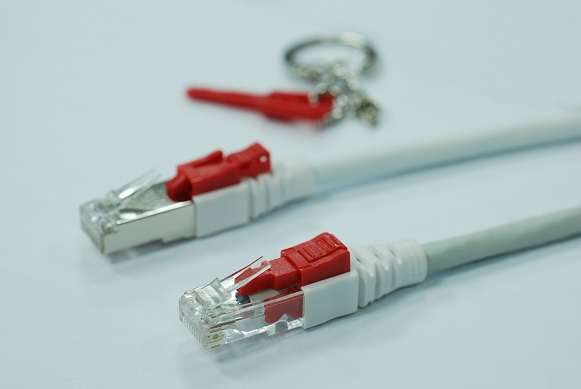
\includegraphics[width=0.5\textwidth]{pics/portsec.jpg}
        \caption[RJ45-lås]{Ett exempel på säkerhetslås för RJ45-kontakter.}
        \label{fig:rj45-caps}
    \end{figure}

\subsection{Admin-access \& Deployment}
    Admin-access kommer att lösas genom autentisering mot RADIUS där en användargrupp är konfigurerade som administratörer och med deras inloggningsuppgifter kan de logga in i alla enheter på alla siter. På enheterna kommer det även finnas ett lokalt konto för administratörer som backup ifall enheten inte kan nå RADIUS-servern. All kommunikation mellan administratörer och enheter sker över SSH version 2 och alla konfigurationstillfällen loggas centralt för att hålla reda på vem som gjort vad och när. \\
    
    \noindent Siterna finns i flera olika länder och utrustningen måste skeppas ner dit. När utrustningen transporteras ska det ej finnas någon konfiguration på dem eftersom paketet kan bli stulet. Skulle paketet bli stulet och det exempelvis är brandväggskonfiguration på enheten kan den som stjäl enheten se hur brandväggen är konfigurerad och då hitta eventuella säkerhetshål in i nätverket. Planen är istället att skicka enheterna till siterna helt tomma, och väl på plats koppla upp dem, ge dem en publik IP-adress för att de ska bli nåbara från en av core-siterna och därifrån skicka färdiga konfigurationer till enheten som läser in detta och sedan är klar för att kopplas ihop med det resterande nätverket.

\subsection{DNS}
    Alla core-siter kommer att ha en DNS-tjänst rullande på samma server som AD, vilket betyder att det kommer vara åtminstone en per core-site och dessa är redundanta mot varandra precis som AD är mellan core-siterna. Skulle mot förmodan alla DNS-servrar gå ner samtidigt kommer användarmaskinerna kopplas mot Fortiguards DNS (En säkerhetsfunktion som ingår i brandväggen) för att kunna ta sig ut på internet.

\subsection{Storm Control}
    Storm control har valts att läggas till som funktion i vår lösning för att det är en enkel och bra lösning som skyddar LAN från DOS-attacker eller dålig nätverkskonfiguration. Trafik som stormar, vare sig det är på grund av en angripare eller felaktig konfiguration, skapar onödig trafik på nätverket och degraderar nätverks prestanda. Konfiguration av Storm control på Fortinet-switchar är globalt på hela switchen och görs genom att specificera en maximal tröskel i paket per sekund (pps) \cite[48]{FN_FortiSwitch-Admin-Guide}. Om denna gräns överstigs blockar switchen några paket från att gå igenom tills pps har blivit mindre än den tillåtna tröskeln.

\subsection{NTP}
    Tidssynkronisering i nätverk är en väldigt viktig del när man ska administrera, säkra och lösa eventuella problem som kan uppstå i ett nätverk. Detta för att de flesta problem kan bara fastställas och lösas när man vet vad som hände och när det hände och utan den exakta tiden är det ofta omöjligt att bestämma var problemet ligger. NTP har valts som protokoll för tidssynkronisering för att det anses vara ett State of the Art tidssynkroniserings-protokoll och tidsförskjutningen är bara någon millisekund över internet och ännu lägre på ett lokalt LAN. NTP-servern är tänkt att bli placerad på core-siterna som sedan de mindre siterna synkroniserar sig emot. På grund av att NTP använder ett hierarkiskt system för synkronisering kan siter som tappar anslutning mot core fortfarande ha rätt tid då den närmsta enheten mot NTP-servern kommer bli ansvarig för synkronisering. Detta är viktigt eftersom tiden fortfarande då är rätt och synkad med andra enheterna i nätverket även när siten inte kan nå core.

\subsection{Loggning}
    Att sätta upp ett bra system för att övervaka och spara loggar i ett nätverk är kritiskt för både administration och säkerhet. I vår lösning har vi tänkt att spara loggar lokalt i 24 timmar för trafik som går igenom routrarna och sedan skicka de loggarna till en central loggserver på core. Om siterna inte kan nå core och ladda upp sin logg för de senaste 24 timmarna ska de sparas lokalt tills de kan kommunicera med core igen. Fortinet-enheter kör FortiOS och det erbjuder en robust loggningsmiljö där man kan övervaka, spara samt rapportera trafik och event som har med brandväggen att göra \cite{FN_FortiGate-Logging}. Man kan både välja att spara lokalt på enheten och skicka till en eller flera loggservrar.

\subsection{DHCP}
    En DHCP-server är tänkt att placeras ut lokalt på varje site för att dela ut IP-adresser för det spann som den siten är tilldelad. Genom att placera en DHCP-servern på varje site istället för på core kommer det leda till att de lokala enheterna på siterna fortfarande kan få en IP-adress tilldelad även om den siten inte kan nå core. FortiGate 60E på varje site kommer att användas som den lokala DHCP servern för att den är enkel att konfigurera och behöver man inte ha någon extra server bara för DHCP.

\newpage
\subsection{Firewall}
    FortiGate har en inbyggd brandvägg med IPS och threat protection \cite{FN_FortiGate-60E}. Med hjälp av FortiGuard kan varje FortiGate snabbt uppdatera dess signaturlistor för kända virus, trojaner och maskar att blockera. FortiGuard har också ett inbyggt App Control-system för eventuella begränsningar av förbjudna program eller tjänster. FortiGate 60E-PoE-modellen kan med alla tjänster aktiverade skyffla 200 Mbps av data, väl tillräckligt för det satta minimikravet.

\subsection{FortiClient}
    FortiClient är Fortinets egna program för end-point-skydd, dvs ett antivirusprogram för klienter \cite{FN_FortiClient}. FortiClient använder FortiGuard för att enkelt kunna uppdatera dess signaturlista. Dock är det upp till användarna att säkra sin utrustning för att vi inte har någon kontroll över deras enheter så vi kan endast rekommendera ett antivirus skydd.

\subsection{RADIUS}
    FortiGates kan enkelt konfigureras så att klienter ska autentisera med vald metod (MS-CHAP, CHAP, PAP) till en RADIUS server. Helst bör ett autentiserat certifikat användas för att säkerställa att RADIUS servern är genuin.

\subsection{NAT}
    NAT används inom hela nätverket då kanske endast ett eller ett fåtal publika IP-adresser finns tillgängliga och alla enheter samt klienter använder privata adresser. Dock behöver siternas routrar inte behandla NAT då enligt vår föreslagna design konverteras all NAT-trafik hos core-siterna innan data skickas ut på publikt internet.

\section{IP-Design}
    Tanken med IP-designen är att använda privata adresser över hela nätverket. Detta på grund av att all trafik från siterna kommer gå över en VPN-länk till Core och därefter ut på nätverket. Detta innebär att hela företagets nät blir ett virtualiserat privat nätverk. För att adressering ska vara så enkel som möjligt blir varje site tilldelad ett löpnummer som representerar den andra oktetten i IP-adressen (ex. 10.\textbf{55}.0.0) vilket då är IP-adressen till site nummer 55. Den tredje oktetten i IP-adressen representerar de olika VLAN som finns på siten (ex. 10.55.\textbf{20}.0) som är IP-adressen för site nummer 55 och VLAN 20. På det här sättet finns det även utrymme för expansion av fler siter då de enkelt kan läggas till utan att IP-planen behöver göras om. Det är också enkelt att avveckla siter och då frigöra det IP-spannet för användning till en annan site.

\subsection{VLAN}
    Det ska finnas minst 5 VLAN på varje site, en för varje typ av användare/enhet som finns på siten. Dessa VLAN är MGMT, User, Office Equipment, Wi-Fi och Guest. Om det finns fler typer kan flera VLAN läggas till. De olika VLAN:en ska inte kunna kommunicera direkt med varandra av säkerhetsskäl med undantag från till exempel User och Office Equipment då det kan vara en användare på User VLAN:et som vill kunna printa ut något. Vi ser ingen anledning till att en Guest användare ska kunna kommunicera med User- eller Office Equipment-VLAN:en. Exempel på IP-adresserna för VLAN:en kan ses i Tabell \ref{table:ip-plan}.

    \begin{table}[htb]
        \centering
        \caption{Exempel på delegering av VLAN}
        \begin{tabular}{|l|l|}
            \hline
            MGMT 				& 10.0.10.0/24 \\ \hline
            User 				& 10.0.20.0/24 \\ \hline
            Office Equipment 	& 10.0.30.0/24 \\ \hline
            Guest 				& 10.0.40.0/24 \\ \hline
            Wi-Fi 				& 10.0.50.0/24 \\ \hline
        \end{tabular}
        \label{table:ip-plan}
    \end{table}

\subsection{Subnetting}
    Eftersom varje VLAN får ett eget spann på 253 användaradresser behöver ytterligare subnetting inte genomföras. Alla siter och enheter har tillräckligt med adresser för att hålla subnettingen enkel och lätt att förstå.
\section{Test}
Testdelen av denna rapport är mer utav av checklista för uppsättning av nya siter, med punkter för vad som ska göras innan miljön sätts upp och vad man bör undersöka för att se till att enheterna fungerar som de ska.

\subsection{Hårdvara}
Här nedan presenteras sådant som är viktigt att tänka på inför driftsättningen av hårdvaran på en ny site. \\
\\
\textbf{Routing \& Switching}
\begin{itemize}[noitemsep]
    \item Är enheterna inkopplade på ett korrekt sätt?
    \item Starta igång enheten och sätt i USB-minnet med start konfigurationen så att enheten kan ta emot resterande konfiguration från core.
    \item Ta emot konfigurationen från core och driftsätt nätverket.
    \item Kan enheterna nå core?
    \item Kan enheterna nå varandra i det lokala nätverket?
    \item Aktivera alla tjänster.
    \item Deaktivera alla oanvända portar.
    \item Plugga alla oanvända portar.
    \item Låsa använda portar med RJ45-lås.
    \item Alla enheter ska vara inmonterade i rackskåp som ska låsas.
\end{itemize}

\noindent \textbf{Wireless}
\begin{itemize}[noitemsep]
    \item Montera Accesspunkterna.
    \item Koppla till routern och lås kontakten.
    \item Gör enheten redo för att ta emot konfiguration från core.
\end{itemize}

\subsection{Funktioner/tjänster}
Här presenteras en checklista för de tjänster som ska startas vid driftsättning av ny site, och vad som är viktigt att funktionstesta under själva driftsättningen. \\
\\
\textbf{IPsec}
\begin{itemize}[noitemsep]
    \item Sätt upp både VPN och GRE-tunnel om möjligheten ges.
    \item Kontrollera att man kan pinga från site till core på båda anslutningarna om båda finns.
    \item Använd Wireshark eller liknande för att undersöka att paket krypteras korrekt.
\end{itemize}

\noindent \textbf{DNS}
\begin{itemize}[noitemsep]
    \item Pinga DNS-servern på core för att se att den är online.
    \item Se till att enheterna kan ta sig till alla backup-DNS:er inklusive den utanför core.
\end{itemize}

\noindent \textbf{DHCP}
\begin{itemize}[noitemsep]
\item Kolla att DHCP-utdelning fungerar.
\item Är IP-adresserna som delas ut korrekta?
\end{itemize}

\noindent \textbf{Firewall}
\begin{itemize}[noitemsep]
    \item Starta brandväggen.
    \item Uppdatera databasen med signaturer och se till att den är aktuell.
    \item Testa att nå ut på internet med program som inte ska nå ut och se till att de blir blockerade korrekt. (ex. Facebook-chatt fungerar, men inte video eller upload/download.)
\end{itemize}


\noindent \textbf{Loggning}
\begin{itemize}[noitemsep]
    \item Fungerar loggningen och skickar den till core.
    \item Om anslutningen till core går ner sparas loggningen lokalt tills den kan skickas igen till core.
    \item Loggas det som ska loggas?
\end{itemize}


\noindent \textbf{RADIUS}
\begin{itemize}[noitemsep]
    \item Se till att allt som använder RADIUS som autentiseringsmetod fungerar ex. 802.1x, SSH.
\end{itemize}

\noindent \textbf{NTP}
\begin{itemize}[noitemsep]
    \item Se till att NTP-servern på core är synkar mot en genuin tidskälla.
    \item Kontrollera att alla enheter har samma tid och är synkroniserade med NTP-servern på core.
\end{itemize}

\noindent \textbf{VLAN}
\begin{itemize}[noitemsep]
    \item Är VLAN-en korrekt uppsatta?
    \item Se till att de VLAN som ska kunna kommunicera kan det och de VLAN som inte ska kunna kommunicera inte kan göra det.
    \item Kolla så att enheter är på rätt VLAN.
\end{itemize}


% ##########

\section{Avslut}
Detta är det lösningsförslag som vi tagit fram och vi hoppas att det ska vara till nytta i framtiden. Vi vill uttrycka ett tack till NetSecure och Johnny för att vi fick ta oss an detta projekt, det har varit både intressant och lärorikt.



% ============================= References ============================
% Comment out these lines if you don't need a list of references.
    \clearpage
    \pagenumbering{roman}
    \printbibliography[heading=bibintoc]

% ============================= Appendices ============================
% Comment out these lines if you don't need a any appendices
    %\clearpage
    %\begin{appendices}
       %\section{Första Bilagan}
En enkel bilaga. Varje sektion skapar en ny bilaga i dokumentet.

\subsection{En subsektion i bilagan}
Exakt vad det står. Blir en del av den redan skapade bilagan.

\section{En annan sektionstitel i första bilagan}
Skapar en ny bilaga.
       %\section{En ny bilaga fil}
Inget mer att se här.
    %\end{appendices}

% ============================ Document End ===========================
\end{document}
